 \documentclass[a4paper]{article}
\usepackage[francais]{babel}
\usepackage{fontspec}
\usepackage{enumitem}
\usepackage{authblk}
\usepackage{minted}
\usepackage{amsmath}
\usepackage{tabularx}
\usepackage{graphicx}
\newcolumntype{C}[1]{>{\centering\arraybackslash}p{#1}}
\graphicspath{{images/}}
\setlength{\parindent}{0pt}
\usepackage[left=2.5cm,top=2.5cm,right=2.5cm,bottom=2.5cm]{geometry}

\title{Projet VHDL}
\author{Mehmed Blazevic \& Orphée Antoniadis}
\date{Hepia 2018}
\begin{document}

\maketitle

\section{Introduction}
Dans le cadre du cours de VHDL, FPGA \& SoPC, il nous a été demandé de réaliser un projet.
Le projet s'étale sur tout le semestre et le thème est libre. Nous avions tout de
même certaines contraites:

\begin{itemize}
  \item Utiliser un périphérique existant (SPI, I2C, UART, ...)
  \item Créer un périphérique spécifique
\end{itemize}

\section{Notre idée}
Nous voulions travailler avec le musique. On pensait faire un instrument un peu
différent de ce que l'on a l'habitude de voir. L'idée est de travailler avec l'espace.
Nous avons décidé d'utiliser des capteurs ultrasons, afin de connaître la distance
entre une main et ce capteur. En fonction de la distance que l'on mesure avec la main,
nous avions dans l'idée de produire une notes de musique plus ou moins forte.
L'idée était de placer 8 capteurs de distances allignés, afin de jouer avec un piano
"virtuel". Cette idée fait penser au thérémine.

\subsection{Schema}

\begin{center}
\noindent\makebox[\textwidth]{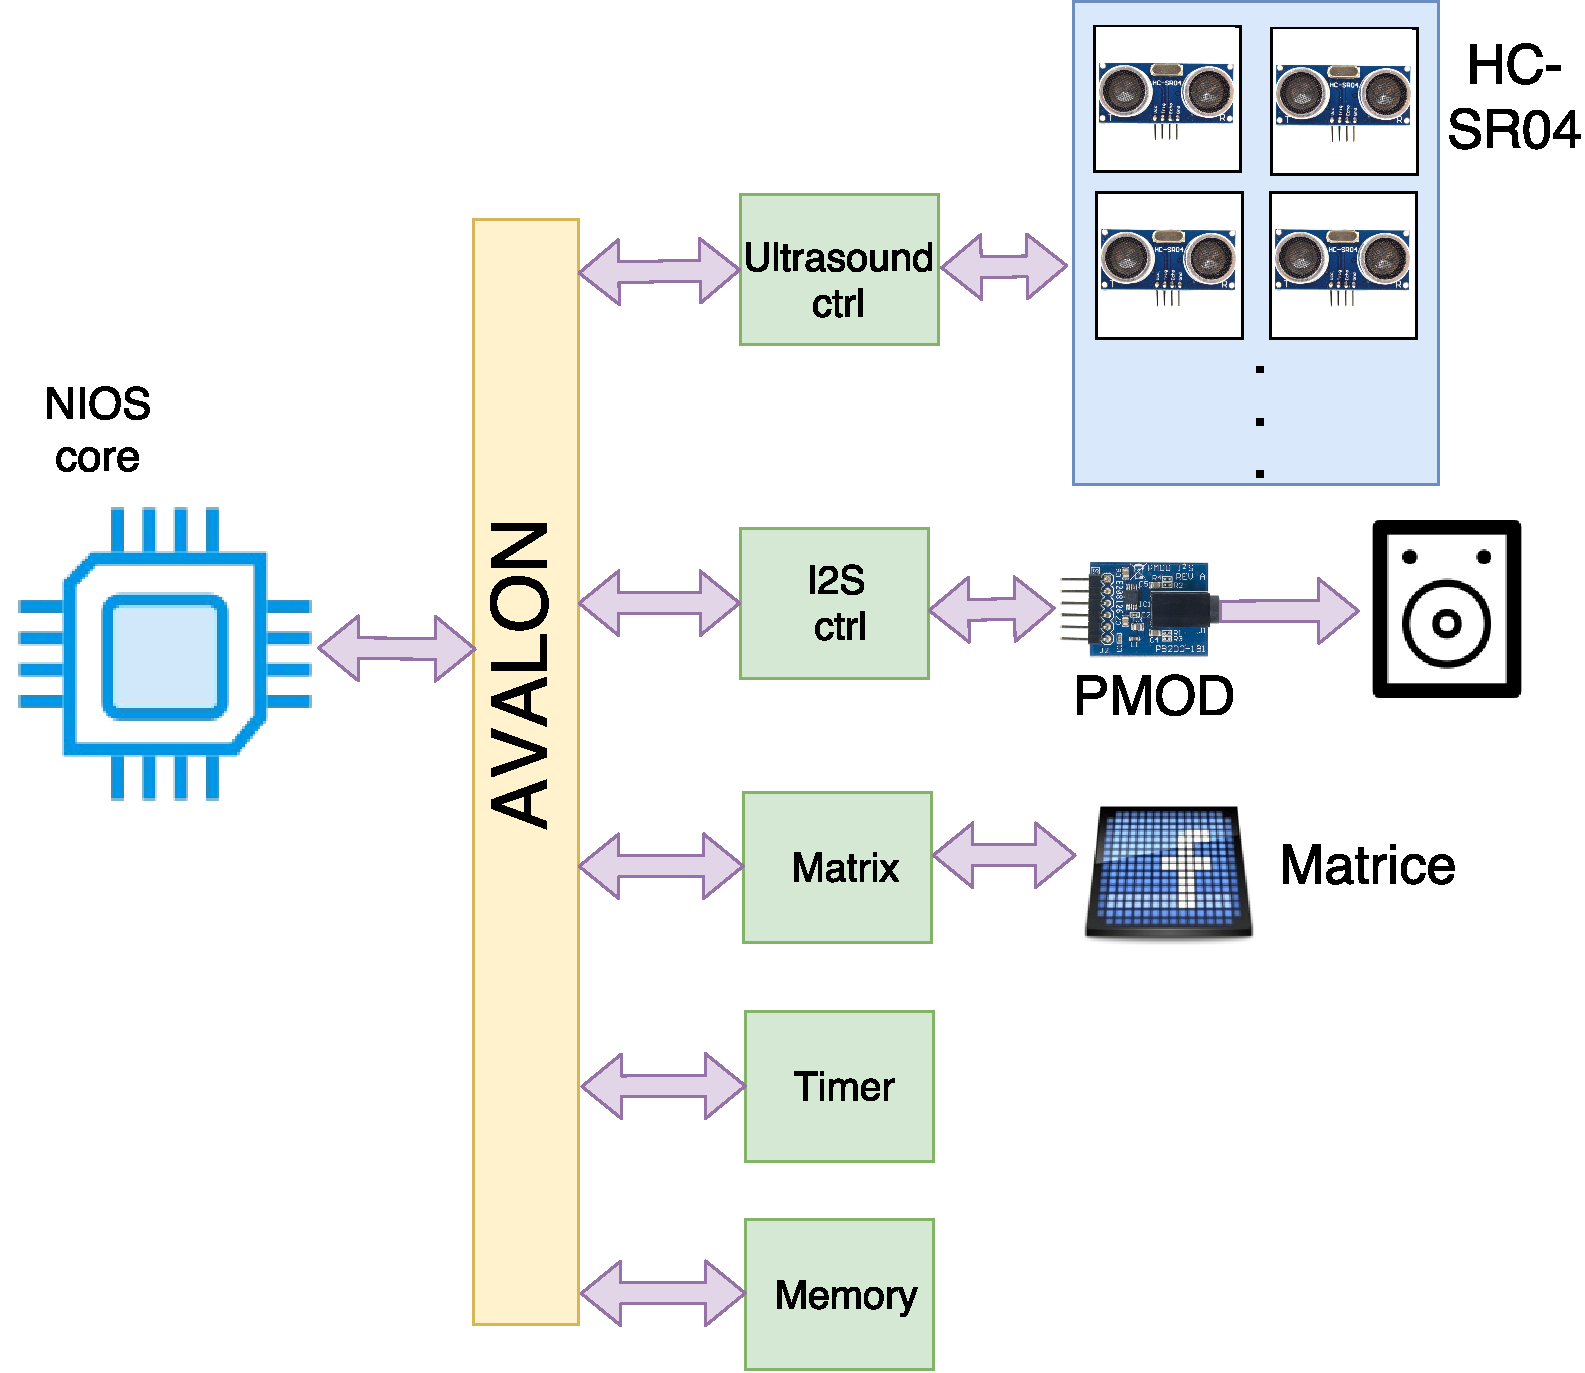
\includegraphics[width=350pt]{VHDL.pdf}}
\end{center}

\section{Drivers}
\subsection{Capteur ultrasons}
Le module ultrason que nous avons utilisé est le HCSR04 de Cytron Technologies.
Ce module est composé de 4 pins, le Vcc, le Gnd, une entrée appelée trig et une
sortie appelée echo. Il utilise son propre protocole qui est très simple. Lorsque l'on
souhaite obtenir la distance, il faut mettre la pin trig à l'état haut pendant
10$\mu$s. Il faut ensuite remettre le trig à l'état bas, le module envoie une onde
ultrason et met la pin echo à l'état haut. L'echo est remis à l'état bas lorsque
l'onde ultrason a fait l'aller-retour. Pour obtenir la distance, il faut donc mesurer
le temps que l'echo a été à l'état haut. A noter que le module ultrason fonctionne
en 5V et la DE0 fonctionne en 3V3. Nous avons donc du faire un petit diviseur de tension
sur la pin echo. Le trig étant une entrée, les 3V3 de la FPGA suffisent à considérer
le signal comme étant à l'état haut. \\

Le driver que nous avons développé reproduit le comportement décrit ci-dessus.
Nous avons utilisé une machine à états pour le reproduire. Pour éliminer le bruit,
nous faison une moyenne sur 100 échantillons. L'interface avalon dévéloppée est
très simple elle aussi. Il n'y a qu'un seul registre en lecture seule. Ce registre
contient le nombre de coups d'horloges de la DE0 pendant lesquels l'echo était à
l'état haut. Au niveau du code C il suffit de convertir ces coups d'horloge et
utiliser la vitesse du son afin d'obtenir la distance entre le module et l'obstacle.
Notre driver fonctionnait mais nous avons remarqué que la distance calculée n'était
pas très précise mais assez pour notre projet.

\subsection{I2S}

Pour la génération des différents sons, nous utilisons un PMODI2S de chez Digilent.
C'est un module qui utilise un DAC CS4344 qui fonctionne avec le protocole I2S. Le DAC
est un composant qui permet de transformer un signal numérique en un signal analogique.
C'est un composant largement utilisé dans l'audio, car le signal analogique créé par le DAC peut
être envoyer directement sur une sortie jack par exemple, comme c'est le cas dans le module que l'on utilise.
Le plus important ici est de maîtriser le protocole I2S. C'est un protocole qui utilise
4 fils:

\begin{itemize}
  \item MCLK : la master clock, nécessaire au fonctionnement
  \item LRCK : left/right clock, permet de choisir la voie (appelé SW ou Fs aussi)
  \item SCK  : la clock pour les datas
  \item SDIN : les datas (appelé SD aussi)
\end{itemize}

Il est très important de respecter les différents timings. C'est un protcole très simple,
mais très exigeant sur les timings. Ci-dessous, on voit la synchronisation entre les différents
éléments.
\begin{center}
\noindent\makebox[\textwidth]{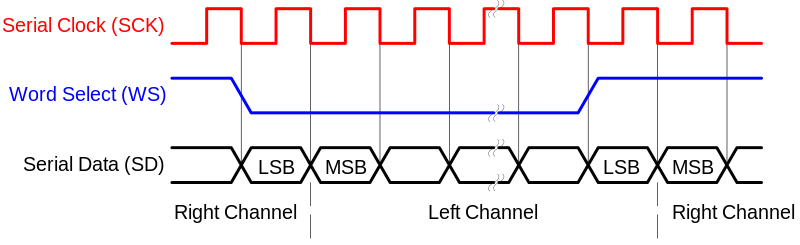
\includegraphics[width=350pt]{timing_is2.png}}
\end{center}

Ici, il manque la clock master MCLK. On peut voir que l'on peut pas envoyer une donnée
n'importe quand. Il faut qu'un envoie de donnée se fasse lorsqu'on change de channel. De plus,
le MSB est envoyé en premier et les données sont des valeurs signées. Le DAC détectera donc
rapidement si on lui envoit une valeur positive ou négative.

\newpage

Pour choisir les fréquences que l'on veut utiliser, il faut se référer au tableau suivant:

\begin{center}
\noindent\makebox[\textwidth]{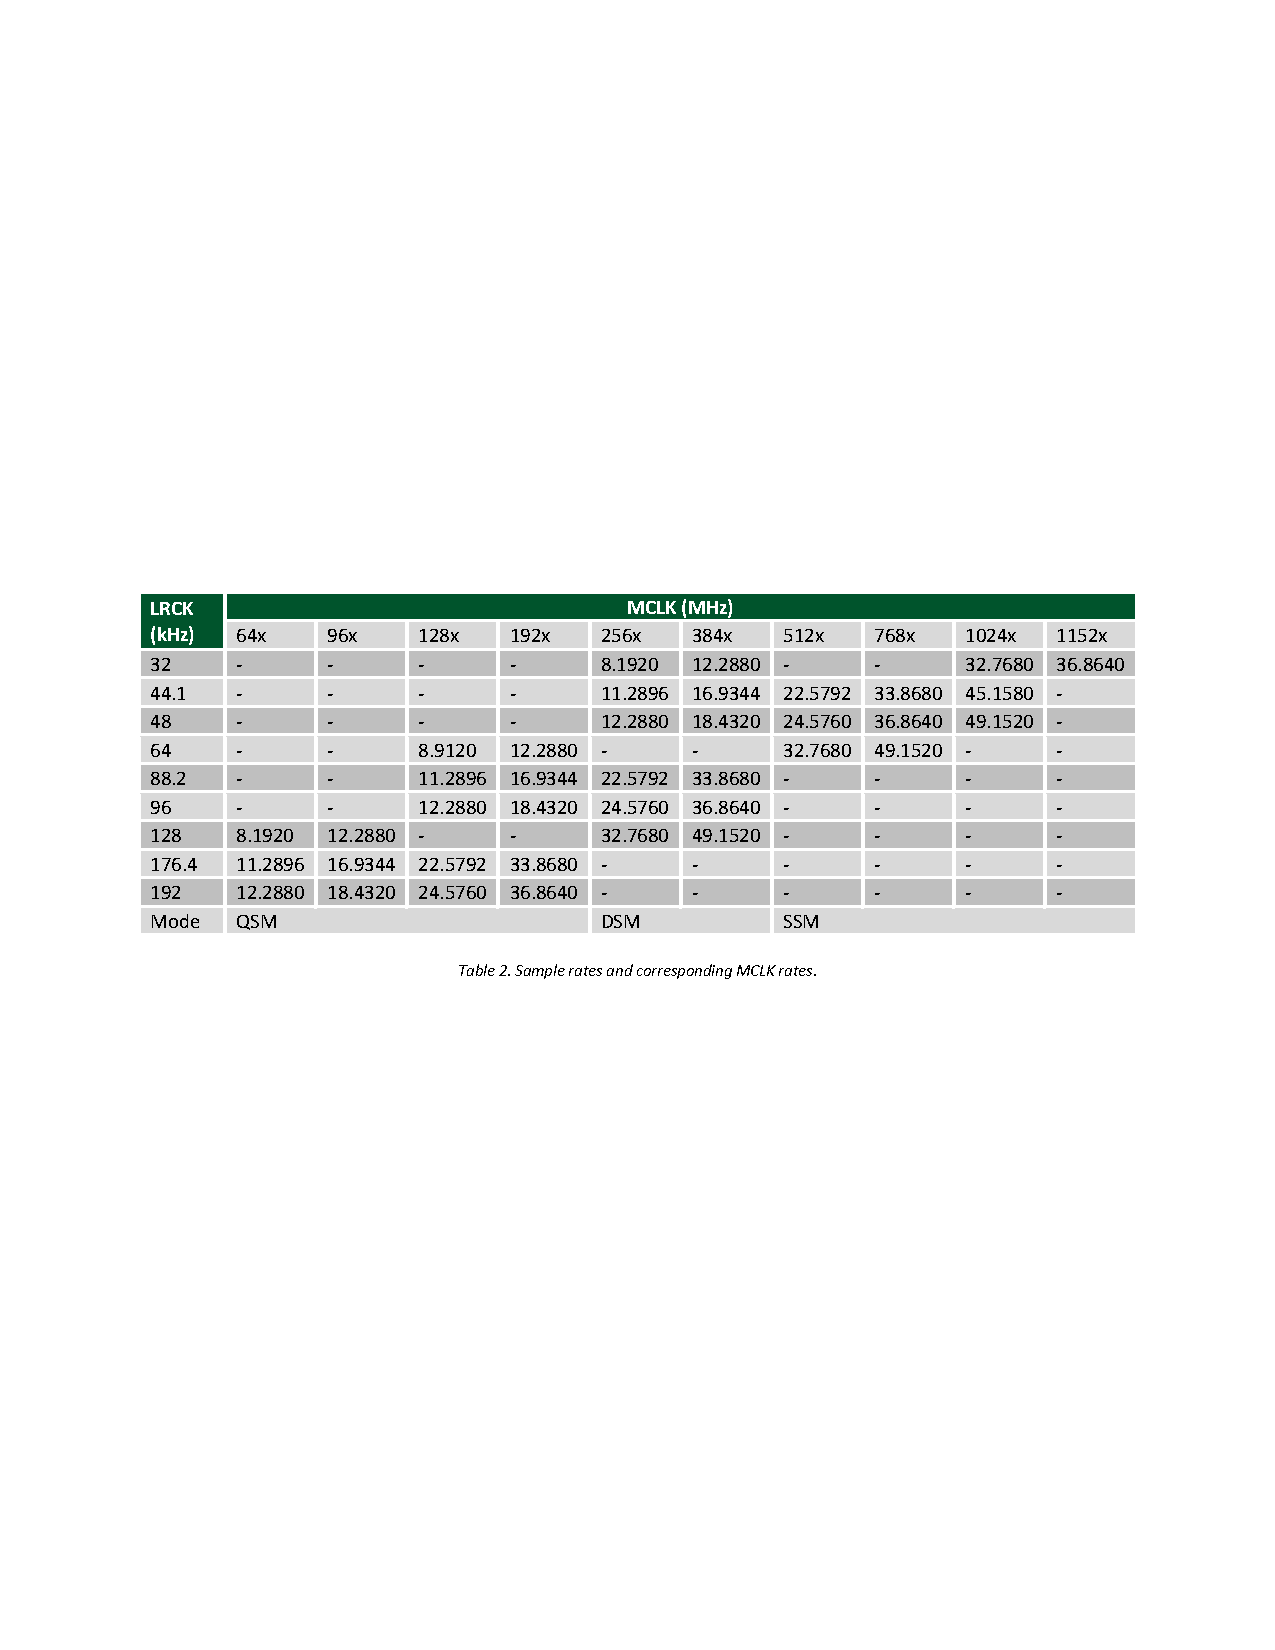
\includegraphics[width=400pt]{table.pdf}}
\end{center}

Il est donc possible de choisir plusieurs valeurs de fréquences. Ici, nous avons choisi,
de façon naïve la première valeur de la première colonne. On se retrouve donc avec:

\begin{itemize}
  \item MCLK à 8.192MHz
  \item LRCK à 128 kHz
\end{itemize}

Pour la clock des données, il faut se référer à:
\begin{center}
\noindent\makebox[\textwidth]{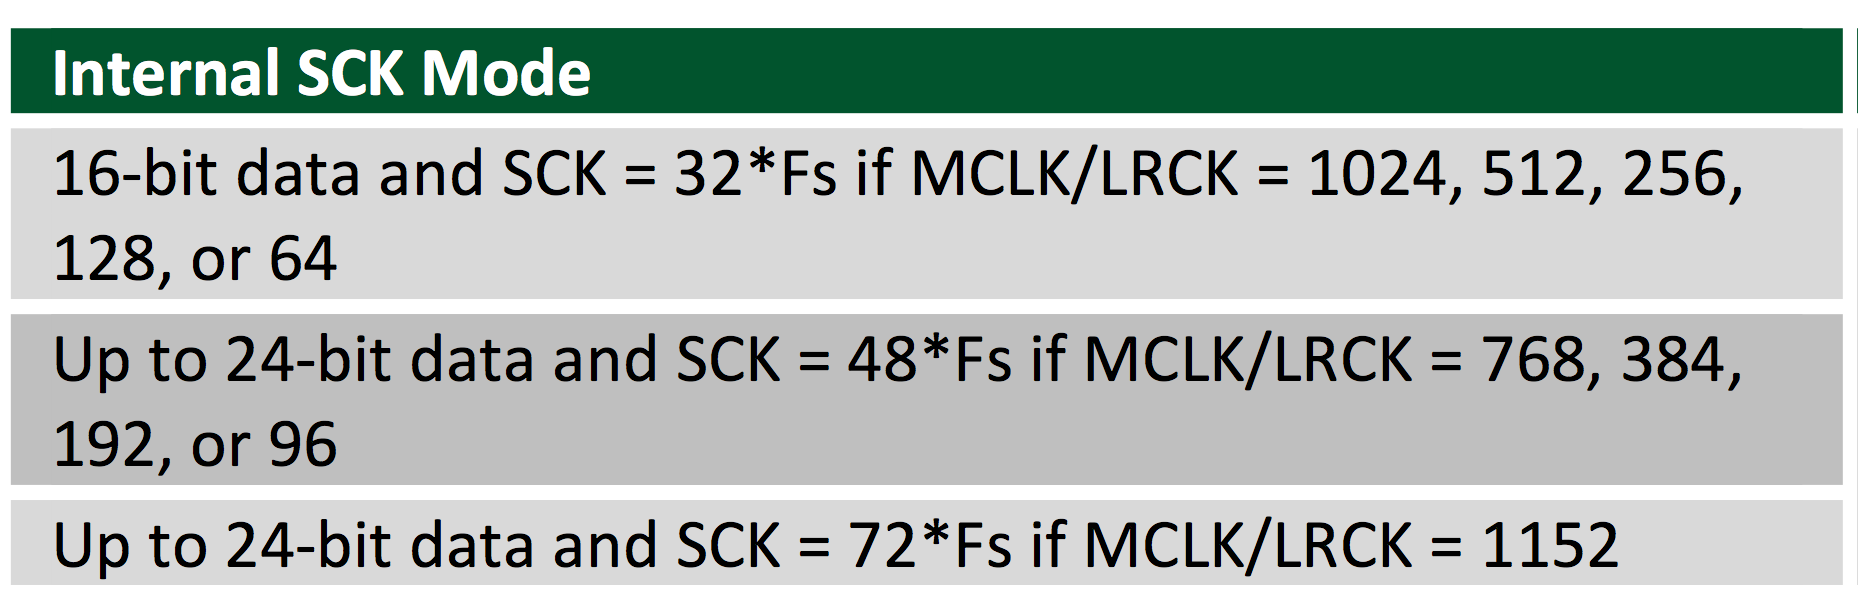
\includegraphics[width=250pt]{dataclock}}
\end{center}
On se retrouve avec SCK = 32*128kHz = 4.096MHz. Il faut que les données soient envoyées à
SCK/2 pour que la clock des données corresponde à la bonne donnée.

Le composant VHDL est prévu pour fonctionner à ces valeurs de clock, mais il est facile
de les changer avec des constantes. Le composant VHDL possède une sortie qui va passer à '1'
lorsque 32 bits sont finis d'envoyer et à ce moment on peut charger une nouvelle valeur
à l'entrée du composant VHDL. Le composant avalon n'est pas très compliqué. Il possède 3 registres:

\begin{itemize}
  \item iRegCtrl: permet de configurer le composant (juste enable pour le moment)
  \item iRegData: le registre des données envoyés au composant I2S
  \item iRegBuffer: le buffer dans lequel écrit le NIOS
\end{itemize}

Nous n'avons pas implémenter l'interruption, mais elle peut l'être en décommentant
2 blocks qui se trouve dans le fichier \textit{i2s\_controller}. Lorsqu'on veut envoyer
une donnée, elle sera envoyée en continue. Elle changera lorsqu'on écrira dans le registre
de buffer.

\subsection{Matrix}
Nous utiliser le driver que l'on a implémenté pour la matrice de leds. Nous nous en servons
pour afficher l'amplitude de chaque note.

\newpage

\section{Fonctionnement}
Le fonctionnement est simple. Lorsque le tout est alimenté, il faut placer sa main au dessus
d'un capteur de distance et un son sera produit. Chaque capteur représente une note.
Pour le moment, nous avons les notes do, si, la, sol.

\section{Conclusion}
Le projet était réellement intéressant à faire. Nous avons beaucoup apprécié passer du temps
dessus. Nous espérons avoir de nouveau l'occasion de participer à un tel projet. Le
projet fonctionne correctement, mis à part les connecteurs qui sont un peu fatigués. Plusieurs
améliorations sont envisageables, comme le calcul des notes par VHDL par exemple.


\end{document}
